\documentclass[paper.tex]{subfiles}

\begin{document}


\section{Proof that $\mathcal{V}$ is a universal template}

In this section we outline the proof given in full detail in~\cite{Ghrist1996} that $\V$ (shown in figure~\ref{fig:universal}) is a universal template. Details will inevitably be omitted but our goal in this exposition is to straddle the line between
the full proof and the very high-level outline given in~\cite{knottyode}, giving a concise and readable exposition that gets at the essence of the proof.

The essential idea is to find a special set of templates which have a special property that forces them to support all braids as orbits, and then to show that these templates can be found in $\V$. Since all knots and links
can be realized as a braid, this immediately implies that $\V$ is universal. The last step of showing that the special braid-supporting templates can found in $\V$ is the most difficult by far and where we will have to do the
most hand-waving. Nonetheless, we will try to capture the essence.

\begin{figure}[h]
  % not sure where to put this, but not here

    %this doesn't seem like too bad of a spot; you mention figure 1 in the first paragraph of this section so it shouldn't be placed too far away from that paragraph
  \centering
  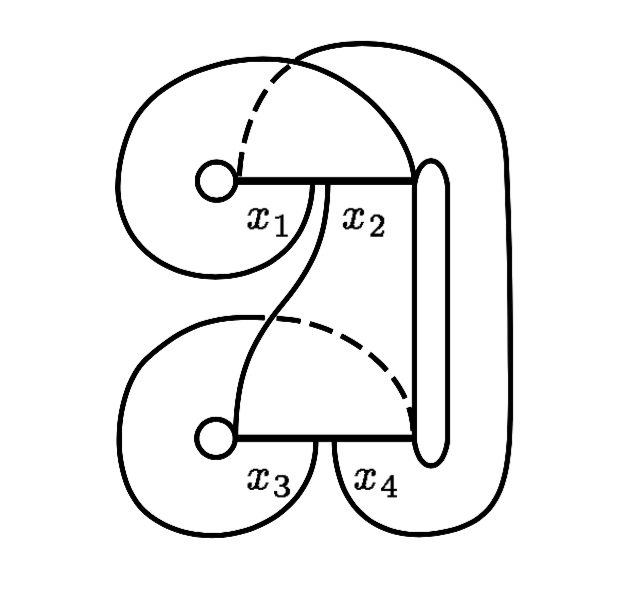
\includegraphics[width=0.5\textwidth]{universal.png}
  \caption{The universal template, reproduced from~\cite{knottyode}}\label{fig:universal}
\end{figure}

\subsection{Braids and the theorem of Alexander}

Recall that a closed braid is a collection of $P$ disjoint simple closed curves in a standardly embedded torus $D^2 \times S^1$ such that every $D^2$ cross-section of the torus intersects the closed braid in exactly $P$ points.

% related to pure braid group/symmetric group -- this following line isn't entirely accurate, so I've commented it out for now
%Braids have a natural identification as a permutation on $P$ elements, which is the property we exploit. 

In a landmark paper~\cite{Alexander1923}, Alexander proved the following theorem which provides the crucial connection
between braids and links.

% we exploit it since each permutation can be written as the product of exchanges

\begin{thm}[Alexander 1923]
  Each knot or link is isotopic to some closed braid on $P$ strands for some $P$
\end{thm}

\subsection{The templates $\W_q$}

The family of templates $\set{\W_q}$ shown in figure~\ref{fig:w_q} are those referred to earlier as the braid-supporting templates. $\W_1$ is identically $\V$ and increasing $q$ by one has the effect of adding
two \emph{ears} to one side. The property that successive ears alternate in `sign' is what makes this family of templates so useful, as this property makes proving that they support all braids delightfully simple.

\begin{figure}[h]
  \centering
  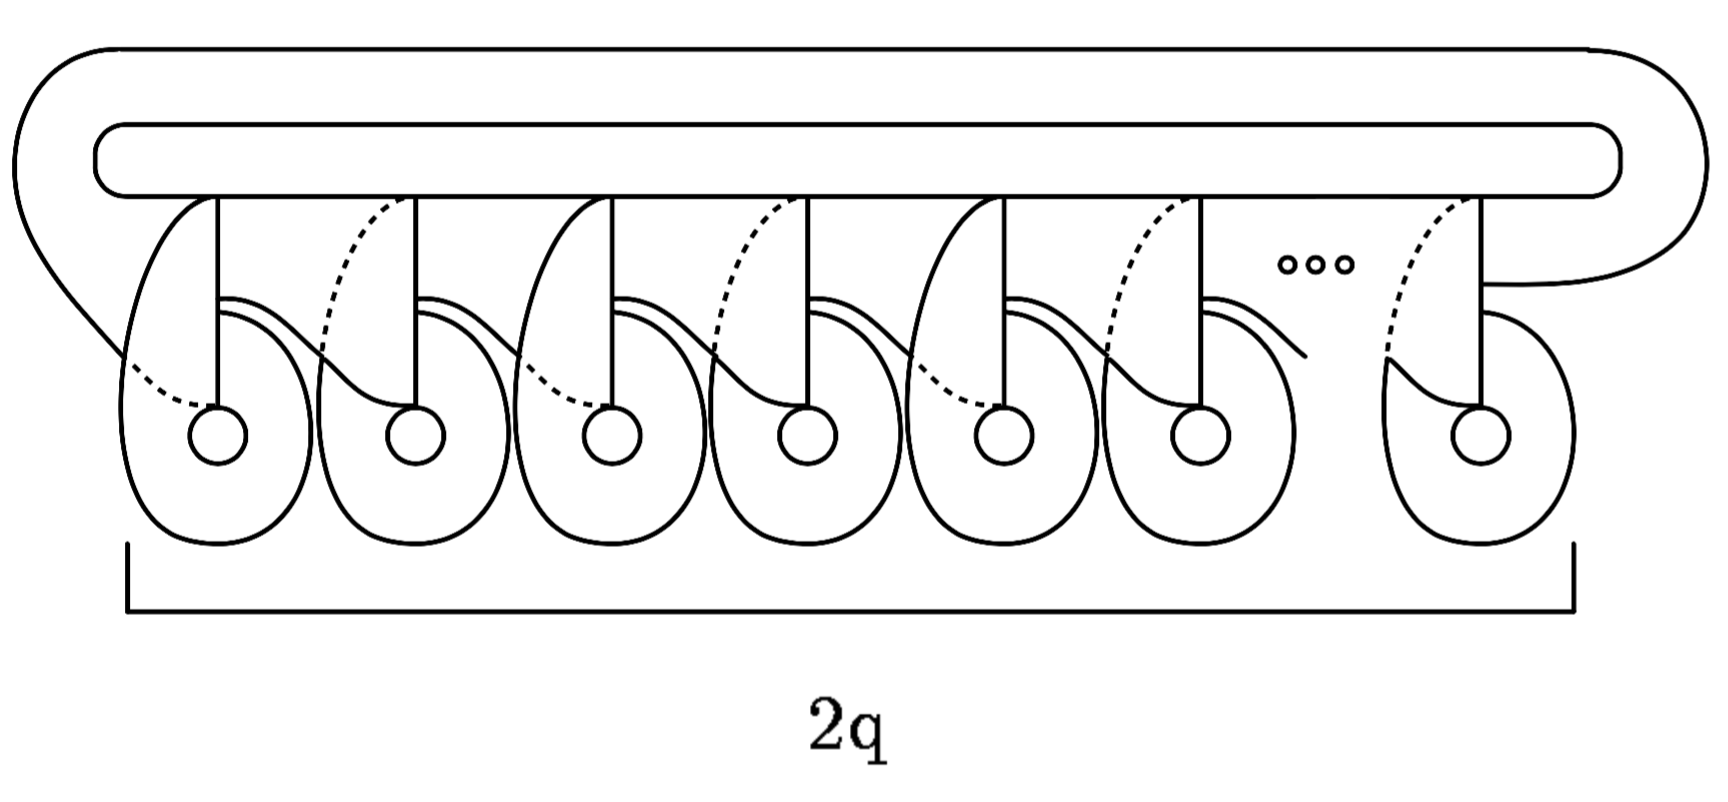
\includegraphics[width=0.8\textwidth]{w_q.png}
  \caption{The templates $W_q$, reproduced from~\cite{knottyode}}\label{fig:w_q}
\end{figure}


\begin{lemma}[Ghrist 1996]
  An isotopic copy of any closed braid exists as a set of periodic orbits on some $W_q$ for sufficently large $q$.
\end{lemma}

\begin{proof}
  Braids have a natural connection to the symmetric group $S_n$. A single braid can be identified with an element $s \in S_n$ (for the elements of the symmetric group are permutations) and the concatenation of succesive braids
  mirrors the group operation on $S_n$. In this way, the concatenation of alternative positive and negative ears on $\W_q$ mimics the group operation on $S_n$. We seek to show that a generating set for $S_n$ can be `fit' onto a
  finite concatenation of alternating ears, as occurs in $\W_q$.

  $S_n$ is generated by $\set{\sigma_1, \ldots \sigma_{n - 1}}$ where $\sigma_i$ transposes the ith and (i+1)th strands of the braid. The $\sigma_i$ are subject to the relations $\sigma_i \sigma_j = \sigma_j \sigma_i$
  for $\abs{i - j} > 1$ and $\sigma_i \sigma_j \sigma_i = \sigma_j \sigma_i \sigma_j$ for $\abs{i - j} = 1$.

  Figure~\ref{fig:earexchange} illustrates how to put the word $\sigma_1 \sigma_2, \ldot \sigma_k$ on a positive ear and $\sigma_1^{-1} \sigma_2^{-1} \ldots \sigma_k^{-1}$ on a negative ear. In particular, we explicitly get
  $\sigma_1$ and $\sigma_1^{-1}$ on respectively positive and negative ears. We proceed by induction, asssuming that we can find the generators $\sigma_1, \sigma_1^{-1}, \ldots \sigma_k, \sigma_k^{-1}$ on a finite sequence
  of ears. We can then construct $\sigma_{k+1}$ and $\sigma_{k+1}^{-1}$ by concatenating additional ears as follows


  \begin{align}
    \sigma_{k+1} &= (\sigma_k^{-1}) \ldots (\sigma_2^{-1})(\sigma_1^{-1})(\sigma_1 \sigma_2 \ldots \sigma_{k+1})
    \sigma_{k+1}^{-1} &= (\sigma_k) \ldots(\sigma_2) (\sigma_1) (\sigma_1^{-1} \sigma_2^{-1} \sigma_{k+1}^{-1})
  \end{align}

  Since we have shown how to construct the words $\sigma_1 \sigma_2 \ldots \sigma_{k+1}$ and $\sigma_1^{-1} \sigma_2^{-1} \sigma_{k+1}^{-1}$ on a single ear, this shows by induction that we can fit the generators for $S_n$ for
  any $n$ on a finite sequence of alternating ears.

  %there's an additional note in the proof given in Ghrist which I don't understand
\end{proof}


\begin{proof}
    %alternate proof? no need for symmetric group I think, and Ghrist don't use that either. I don't think it fits, esp. because going from braid group to symmetric group loses the over/under crossing information and other twists/turns. 

    The concatenation of alternating positive and negative ears on $\W_q$ mimics the braid group concatenation operation. The braid group $B_{n+1}$ is naturally generated by $\sigma_1, \sigma_2, \dots, \sigma_{n}$, where $\sigma_i$ is a single crossing of the $i$th strand over the $(i + 1)$th strand and its inverse, $\sigma_i^{-1}$, is a single crossing of the $(i + 1)$th strand over the $i$th strand. Naturally, $\sigma_i \sigma_i^{-1} = \sigma_i^{-1} \sigma_i = I$. We can consider the elements $\pi_1, \pi_2, \dots, \pi_n, \pi_1', \pi_2', \dots, \pi_n'$ of $B_{n+1}$, where $\pi_i = \sigma_1 \sigma_2 \cdots \sigma_i$ and $\pi_i' = \sigma_1^{-1} \sigma_2^{-1} \cdots \sigma_i^{-1}$. Note that $\pi_1 = \sigma_1$, $\pi_1' = \sigma_1^{-1}$, and that for $i > 1$, 
    
    \begin{align*}
        \pi_{i-1}^{-1} \pi_i  &= (\sigma_1 \sigma_2 \dots \sigma_{i - 1})^{-1} \sigma_1 \sigma_2 \cdots \sigma_i \\ 
                              &= \sigma_{i - 1}^{-1} \cdots \sigma_2^{-1} \sigma_1^{-1} \sigma_1 \sigma_2 \cdots \sigma_i \\
                              &= \sigma_{i - 1}^{-1} \cdots \sigma_2^{-1} \sigma_2 \cdots \sigma_i \\
                              &= \sigma_{i - 1}^{-1} \sigma_{i - 1} \sigma_i  \\
                              &= \sigma_i \\ \\
        \pi_{i-1}'^{-1} \pi_i'  &= (\sigma_1^{-1} \sigma_2^{-1} \dots \sigma_{i - 1}^{-1})^{-1} \sigma_1^{-1} \sigma_2^{-1} \cdots \sigma_i^{-1} \\ 
                                &= \sigma_{i - 1} \cdots \sigma_2 \sigma_1 \sigma_1^{-1} \sigma_2^{-1} \cdots \sigma_i^{-1} \\
                                &= \sigma_{i - 1} \cdots \sigma_2 \sigma_2^{-1} \cdots \sigma_i^{-1} \\
                                &= \sigma_{i - 1} \sigma_{i - 1}^{-1} \sigma_i^{-1}  \\
                                &= \sigma_i^{-1} \\ \\
    \end{align*}

    We can conclude that the elements $\pi_1, \pi_2, \dots, \pi_n, \pi_1', \pi_2', \dots, \pi_n'$ of $B_{n+1}$ are a generating set for $B_{n+1}$. 

    %it's possible to split this proof into two, one half for proving the above is a generating set for B_{n+1} and second half for concluding that W_q contains all braids for large q

    For the braid group $B_{n+1}$, notice that for all $1 \leq i \leq n$, $\pi_i$ can be drawn on any positive ear of $\W_q$, letting all but the bottom strand take the top strip and forcing the bottom strand to take the bottom strip, cross over exactly $i$ strands, and take the top strip. Similarly, for all $i \leq i \leq n$, $\pi_i'$ can be drawn on any negative ear of $W_q$, letting all but the bottom strand take the top strip, forcing the bottom strand to take the bottom strip, cross under exactly $i$ strands, and take the top strip. Examples of $\pi_2$ and $\pi_2'$ of the braid group $\B_5$ are drawn in Figure~\ref{fig:earexchange}. 

    Because this set of elements generates the braid group $B_{n+1}$, any braid $B \in B_{n+1}$ can be drawn as a sequence of $\pi_i$ and $\pi_i'$. If $B$ can be represented with $m$ of these elements, then the closure of $B$ lies in $W_m$, as $W_m$ contains $m$ pairs of positive/negative ears that can each support a $\pi_i$ or $\pi_i'$ structure. Thus, any closed braid on $N$ strands lies in $W_q$ for sufficiently large $q$. 

\end{proof}



\begin{figure}[h]
  \centering
  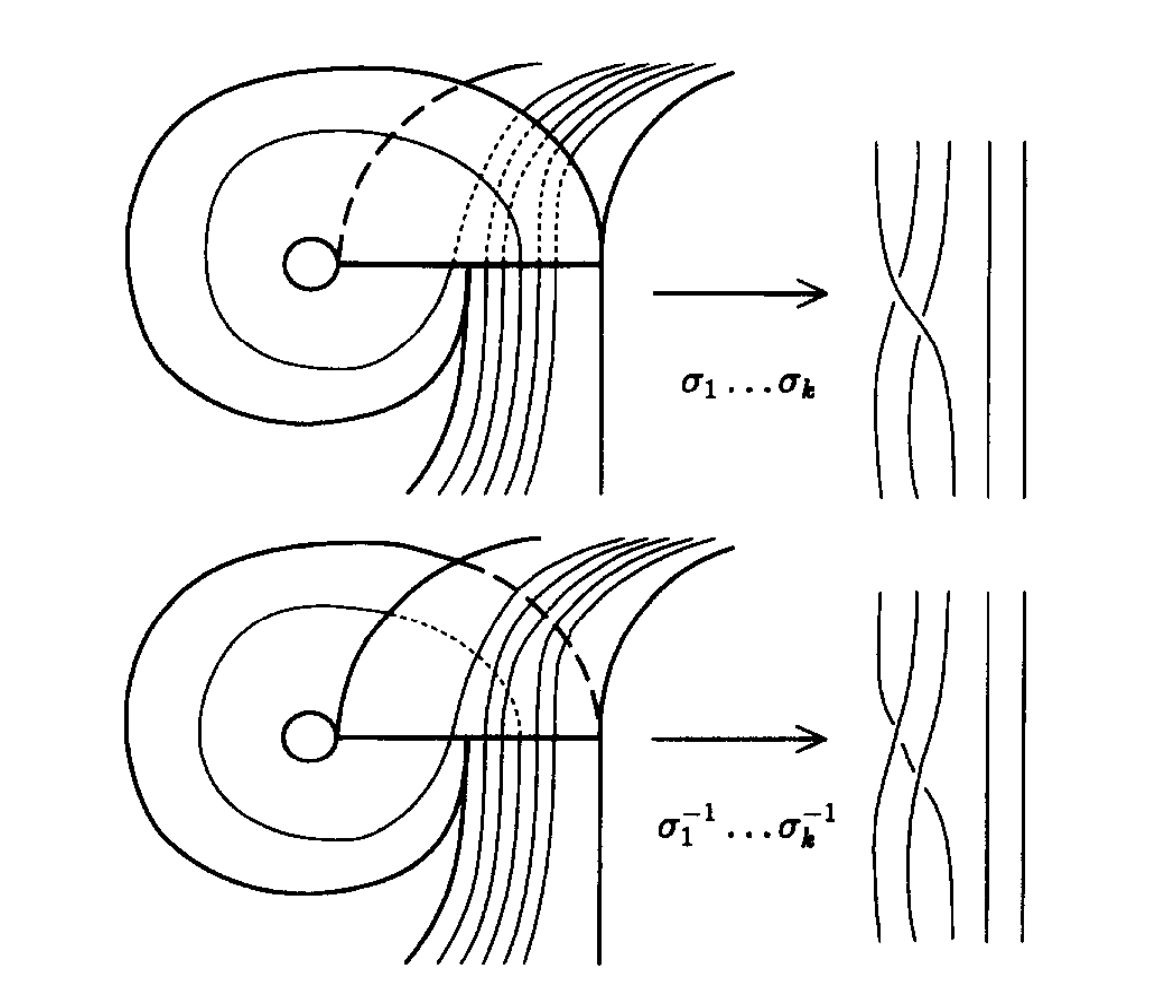
\includegraphics[width=0.8\textwidth]{ear_exchange.png}
  \caption{Top: $\pi_2$ in $B_5$ Bottom: $\pi_2'$ in $B_5$. Figure reproduced from~\cite{Ghrist1996}}\label{fig:earexchange}
\end{figure}




\subsection{Construct $\W_{q+1}$ from $\W_q$}

Start with renormalized $\W_1 \in \V$, and append a pair of ears to\dots

% is this actually necessary?

\subsection{Find $\W_q \subset \V$ for all $q$}

\begin{proof}
    % less handwavy? Still somewhat, but less so. 
    Given that a subtemplate of $\V$ doesn't contain $x_1^\infty$, it is possible to add an ear near the top branch line, like that in Figure~\ref{fig:appendToV}, which is a positive ear. Similarly, given that a subtemplate of $\V$ doesn't contain $X_3^\infty$, it is possible to add an ear near the bottom branch line, which is a negative ear. 

    Let us begin with $\W_1 = \V$. We introduce an renormalization from $\V$ onto $\V$: 
    $$\mathfrak{H}: \V \hookrightarrow \V \begin{cases}
        x_1 \rightarrow x_2 x_3^2 x_4 x_1 (x_2 x_4)^2 x_2 x_3 x_4 x_1 \\
        x_2 \rightarrow x_2 x_3^2 x_4 x_1 (x_2 x_4)^3 x_2 x_3 x_4 x_1 \\
        x_3 \rightarrow x_2 x_3^2 x_4 x_1  x_2 x_4  \\
        x_4 \rightarrow x_2 x_3^2 x_4 x_1  x_2 x_4  \end{cases} $$

        This renormalization satisfies the condition that this subtemplate does not contain $x_1^\infty$. Then, after performing this renormalization, we will be able to add a positive ear at the top branch line; after doing so, we now have $\W_1^+$. 

        There exists a very similar renormalization $\mathfrak{H}^*$ from $\V$ onto $\V$ that will allow us to add a negative ear at the bottom branch ilne. Now, we have added a positive ear and a negative ear, and thus we are now at $\W_2$, yet this subtemplate is still contained within $\V$; thus, $\W_2 \subset \V$. Now, we can repeat this procedure, adding another positive and negative ear after the respective renormalizations to get $\W_3$. 

        This procedure can be repeated $q$ times to show that $\W_q \subset \V$; thus, by letting $q$ approach infinity, $\W_q \subset \V$ for all $q$. 


    \end{proof}


\begin{proof}

    %weird proof. 
    First, we must map $\V$ into itself in such a way that avoids certain edges; see the left diagram of Figure~\ref{fig:appendToV}. After appending the appropriate ears, we send $\V$ back into itself to allow ourselves to iterate this procedure. 

    We start with $\W_1 = \V$ and append two ears (one positive and one negative) to $\W_1$ to get $\W_2$; using the procedure above, we can show that $\W_2 \subset \V$. This can be iterated infinitely many times to show that $\W_q \submset \V$ for all $q$. 
\end{proof}



\begin{figure}[h]
    \centering
    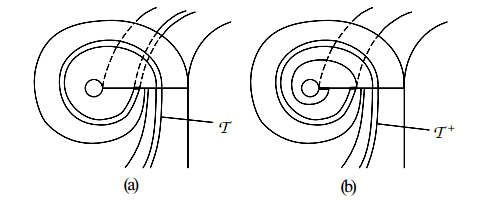
\includegraphics[width=0.8\textwidth]{appendToV.png}
    \caption{Appending a positive ear to $T$ (left) yields $T^+$ (right). Figure reproduced from~\cite{Ghrist1995}} \label{fig:appendToV} %%%%%%%%%%%%%%%%%%%%% link below. 
\end{figure}



%https://www.math.upenn.edu/~ghrist/preprints/eraams.pdf

\subsection{Universal Templates and V}

\begin{thm}[Ghrist 1995]
    The template $\V$ contains an isotopic copy of every tame knot and link as a periodic orbit of the semiflow. 
\end{thm}
\begin{proof}
    This proof comes immediately following the fact that $\W_q \subset \V$ for all $q$, and that all closed braids (and thus all tame links and knots) can be contained within $\W_q$ for large enough $q$. Thus, $\V$ contains every tame knot and link. 
\end{proof}


Ghrist then extends the theorem above to prove the following: 

\begin{thm}[Ghrist 1995] 
    The template $\V$ contains all orientable templates as subtemplates of $\V$. 
\end{thm}

It must follow that if there are any other universal templates $T$, then $\V$ must contain $T$ as a subtemplate. As $T$ contains all tame links and knots as well, as it is universal, the same theorems can be applied to $T$ as were applied to $\V$, so that $T$ also contains all templates (including $\V$). 









\end{document}
